We will now set up the Hartree-Fock equations by varying the coefficients of the single-particle functions.
The single-particle basis functions are defined as
\[
    \psi_p = \sum_{\lambda} C_{p\lambda} \psi_{\lambda}.
\]
where in our case $p=1,2,3,4$ and $\lambda = 1, 2, 3, 4$, that is the first four lowest single-particle orbits of Fig.~\ref{fig:schematic}.
Set up the Hartree-Fock equations for this system by varying the coefficients $C_{p\lambda}$ and solve them for values of $g \in [-1, 1]$.
Comment your results and compare with the exact solution.
Discuss also which diagrams in Fig.~\ref{fig:diagrams} that can be affected by a Hartree-Fock basis.
Compute the total ground state energy  using a Hartree-Fock basis and comment your results.

We will now study the system using non-degenerate Rayleigh-Schr\"odinger perturbation theory to third order in the interaction.
If we exclude the first order contribution, all possible diagrams (so-called anti-symmetric Goldstone diagrams) are shown in Fig.~\ref{fig:diagrams}.
\begin{figure}[hbtp]
    \centering
    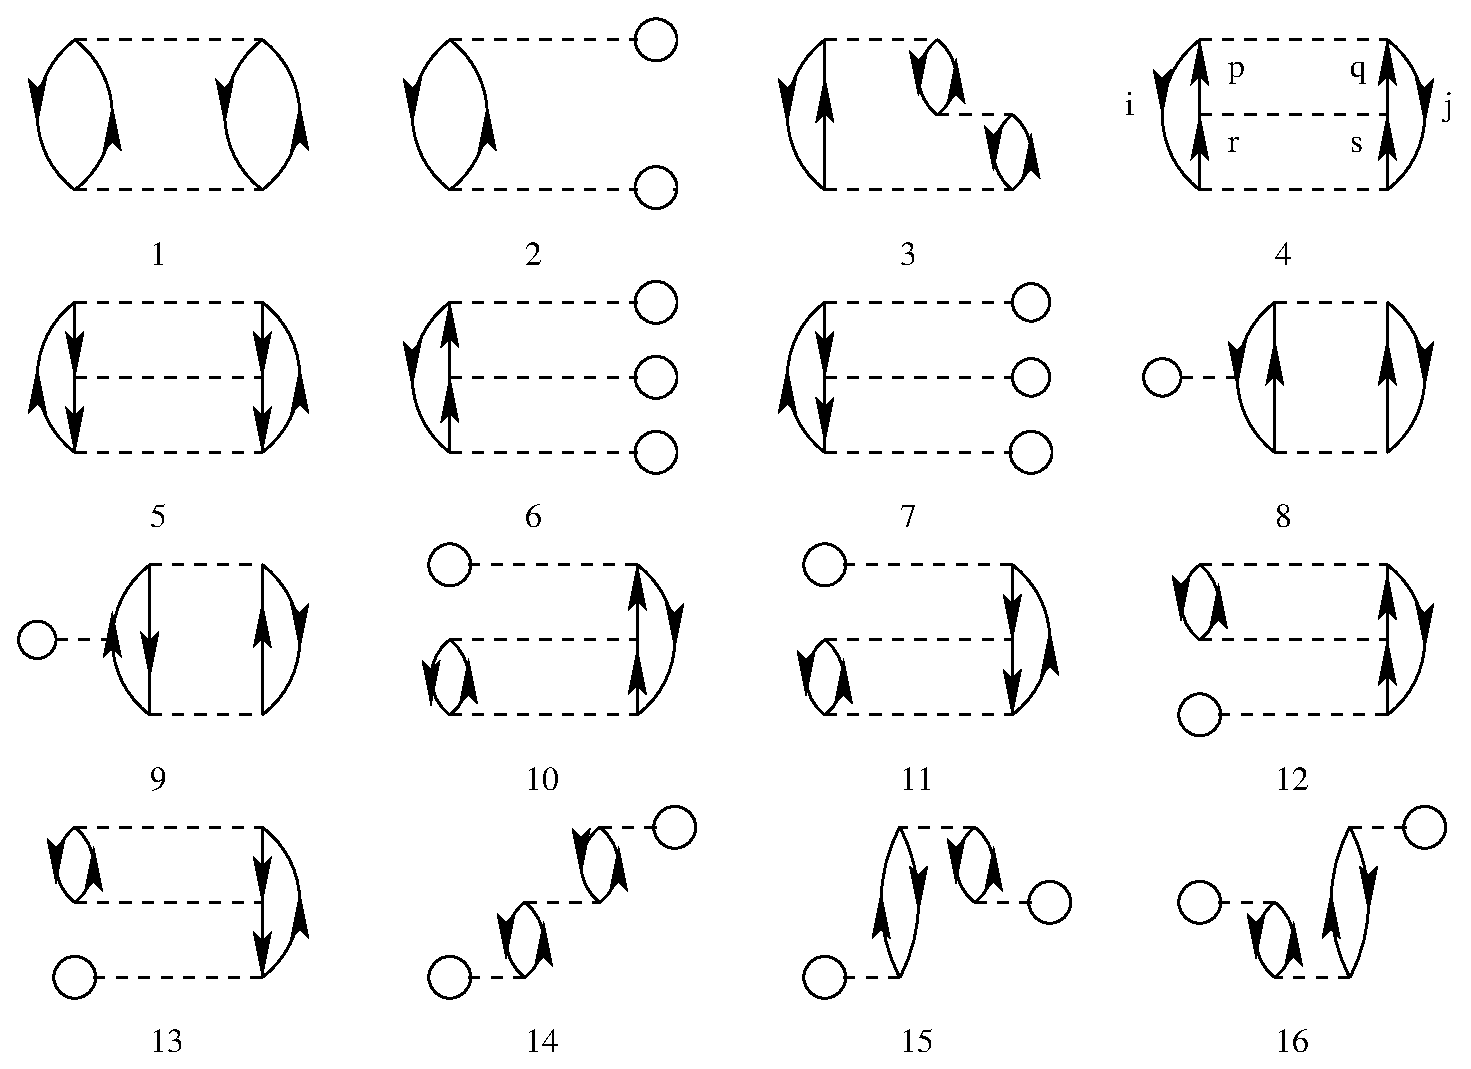
\includegraphics[width=.6\textwidth]{figures/diagrams.eps}
    \caption{
        Diagrams to third order in the interaction.
        The first order
        term is excluded.
        All interaction vertices represent anti-symmetrized matrix elements.\label{fig:diagrams}
    }
\end{figure}

Based on the form of the interaction, which diagrams contribute to the energy of the ground state?  Write down the expressions for the diagrams that contribute and find the contribution to the ground state energy as function $g\in [-1,1]$.
Comment your results.
Compare these results with those you obtained in 2) and 3). % chktex 9 % chktex 10 % tex-fmt: skip

\subsection{}
\subsubsection*{Hartree-Fock}
In the previous midterm, we found that the Hartree-Fock equations by way of varying coefficients are
\begin{equation*}
    \sum_{\gamma} h_{\alpha\gamma}^\HF C_{p\gamma} = \varepsilon_p C_{p\alpha},
\end{equation*}
where the Hartree-Fock matrix elements are
\begin{equation*}
    h_{\alpha \gamma}^\HF = \expval{\alpha}{\hat{h}_0}{\gamma} + \sum_{\beta\delta} \rho_{\beta\delta} \expval{\alpha\beta}{V}{\gamma\delta}.
\end{equation*}

In order to simplify the calculations, we begin by computing the matrix elements of the one-body operator $\hat{h}_0$.
As computed previously, we have that
\begin{equation*}
    \expval{\alpha}{\hat{h}_0}{\gamma} = \delta_{\alpha\gamma} (\alpha - 1).
\end{equation*}
Next, we need to compute the matrix elements of the two-body operator $V$.
We require that the energy levels of bra and ket states match within, and that the spins differ.

Writing $\bar{\alpha}$ as the quantum number with the same energy level as $\alpha$ but with opposite spin, we have that
\begin{align*}
    h_{\alpha\gamma}^\HF &= \delta_{\alpha\gamma} (\alpha - 1) + \rho_{\bar{\alpha}\bar{\gamma}} \expval{\alpha\bar{\alpha}}{V}{\gamma\bar{\gamma}} \\
    &= \delta_{\alpha\gamma} (\alpha - 1) - \rho_{\bar{\alpha}\bar{\gamma}} \frac{1}{2} g.
\end{align*}

We choose our initial guess for the coefficients to be the identity matrix, $C_{p\lambda} = \delta_{p\lambda}$, or equivalently $C = I \in \mathbb{C}^{8 \times 8}$.
We then solve the Hartree-Fock equations for $g \in [-1, 1]$.

Because of our initial guess for the coefficients, we have that the density matrix is
\begin{equation*}
    \rho = C^* C^T = I^* I^T = I.
\end{equation*}
This means that the Hartree-Fock matrix is initially entirely diagonal, with diagonal elements $\alpha - 1 - \frac{1}{2} g$.
As the matrix is diagonal, the eigenvalue problem is already solved, with
\begin{equation*}
    \varepsilon_p = p - 1 - \frac{1}{2} g,
\end{equation*}
where $p$ denotes the energy level, regardless of spin.
We realized this after having implemented a solver, in the file \verb|hartree_fock.py|.

As the coefficients are the identity matrix, we have that
\begin{equation*}
    E[\Phi^\HF] = E[\Phi_0] = 2 - g.
\end{equation*}
As we see in Figs.~\ref{fig:hf_energy} and~\ref{fig:hf_diff}, the Hartree-Fock approximation serves as a poor approximation to the exact solution, with the difference in energy increasing as $|g|$ increases.
However, as it is also a variational method, the energy from the Hartree-Fock calculations will always be higher than the exact energy.
The diagrams in Fig.~\ref{fig:diagrams} that can be affected in the canonical Hartree-Fock case are diagrams 1, 3, 4, and 5.

\begin{figure}
    \centering
    \begin{subfigure}[b]{0.45\textwidth}
        \centering
        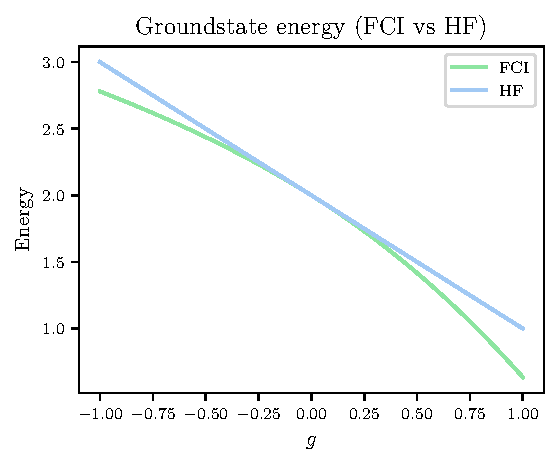
\includegraphics[width=\textwidth]{figures/e_groundstate_energy.pdf}
        \caption{
            Groundstate energy from HF.\label{fig:hf_energy}
        }
    \end{subfigure}
    \hfill
    \begin{subfigure}[b]{0.5\textwidth}
        \centering
        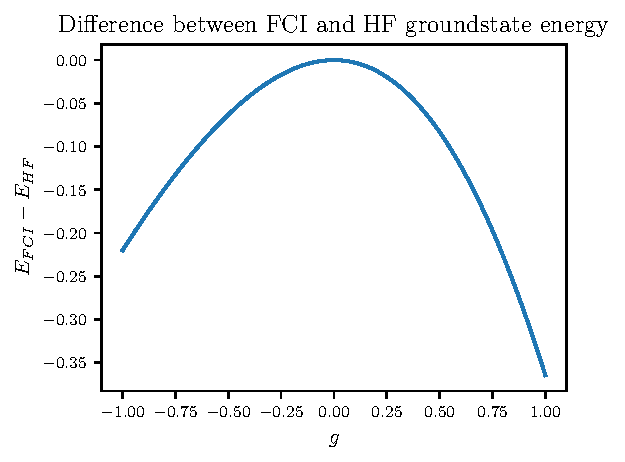
\includegraphics[width=\textwidth]{figures/e_groundstate_energy_diff.pdf}
        \caption{
            Difference in energy from HF.\label{fig:hf_diff}
        }
    \end{subfigure}
    \caption{
        Groundstate energy from the Hartree-Fock calculations, compared with the FCI results, as a function of $g$.
    }
\end{figure}
% \begin{figure}
%     \centering
%     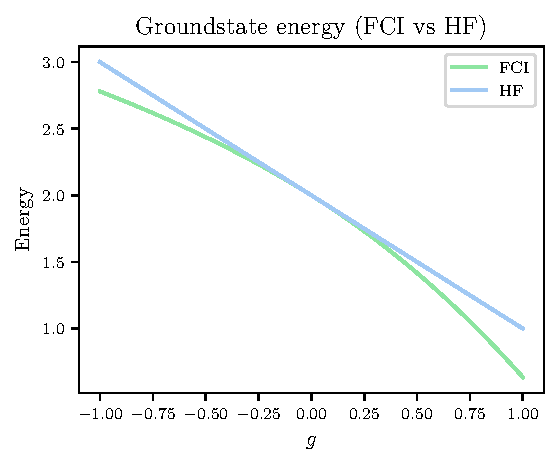
\includegraphics{figures/e_groundstate_energy.pdf}
%     \caption{
%         Groundstate energy from the Hartree-Fock calculations, compared with the FCI results, as a function of $g$.\label{fig:hf_energy}
%     }
% \end{figure}

% \begin{figure}
%     \centering
%     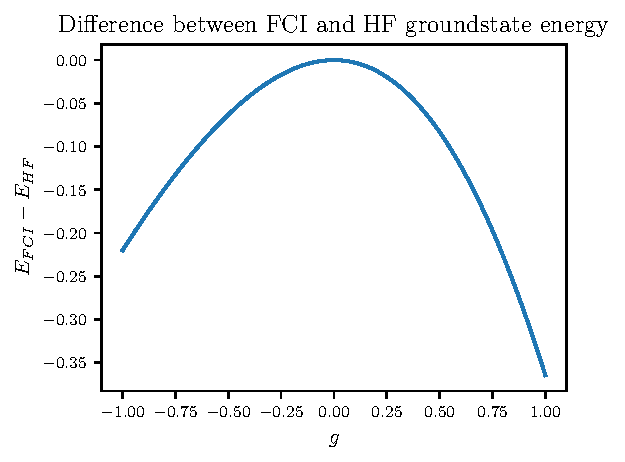
\includegraphics{figures/e_groundstate_energy_diff.pdf}
%     \caption{
%         Difference in groundstate energies of $E_{FCI}$ and $E_{HF}$, as a function of $g$.\label{fig:hf_diff}
%     }
% \end{figure}

\subsubsection*{Rayleigh-Schr\"odinger Perturbation Theory}
We consider now Rayleigh-Schr\"odinger perturbation theory.
For a diagram to be considered possible, we require that no pairs are broken.
We can thus eliminate all diagrams but 1, 4, 5, and 8. % and 9.

As equations, the first diagram contains $n_h = 2$ hole lines, $n_l = 2$ loops, and $n_{ep} = 2$ equivalent pairs.
We thus get a factor of
\begin{equation*}
    \frac{(-1)^{n_h + n_l}}{2^{n_{ep}}} = \frac{(-1)^{2+2}}{2^2} = \frac{1}{4}.
\end{equation*}
The expression for diagram 1 is then
\begin{equation*}
    \frac{1}{4} \sum_{abij} \frac{
        \langle ij \lvert V \rvert ab \rangle
        \langle ab \lvert V \rvert ij \rangle
    }{\varepsilon_i + \varepsilon_j - \varepsilon_a - \varepsilon_b}
    =
    \frac{1}{4} \sum_{ai} \frac{
        \langle i \bar{i} \vert V \vert a \bar{a} \rangle % chktex 7
        \langle a \bar{a} \vert V \vert i \bar{i} \rangle % chktex 7
    }{2(\varepsilon_i - \varepsilon_a)}
\end{equation*}
We have that
\begin{equation*}
    \varepsilon_i - \varepsilon_a = \left( i - 1 - \frac{1}{2} g \right) - \left( a - 1 - \frac{1}{2} g \right) = i - a,
\end{equation*}
so the expression simplifies to
\begin{equation*}
    \frac{1}{4} \sum_{ai} \frac{
        (-\frac{1}{2} g)(-\frac{1}{2} g)
    }{2(i - a)} = \frac{1}{32} \sum_{ai} \frac{g^2}{i - a}.
\end{equation*}

For diagram 4 we have $n_h = 2$, $n_l = 2$ and $n_{ep} = 3$.
The expression is then
\begin{align*}
    \frac{1}{8} \sum_{\substack{abcd \\ ij}} \frac{
        \langle ij \vert V \vert cd \rangle
        \langle cd \vert V \vert ab \rangle
        \langle ab \vert V \vert ij \rangle
    }{
        (
            \varepsilon_i + \varepsilon_j - \varepsilon_a - \varepsilon_b
        )(
            \varepsilon_i + \varepsilon_j - \varepsilon_c - \varepsilon_d
        )
    }
    &= \frac{1}{8} \sum_{aci} \frac{
        \langle i\bar{i} \vert V \vert c\bar{c} \rangle % chktex 7
        \langle c\bar{c} \vert V \vert a\bar{a} \rangle
        \langle a\bar{a} \vert V \vert i\bar{i} \rangle % chktex 7
    }{
        4(
            \varepsilon_i - \varepsilon_a
        )(
            \varepsilon_i - \varepsilon_c
        )
    } \\
    &= \frac{1}{32} \left( -\frac{1}{2} \right)^3 \sum_{aci} \frac{
        g^3
    }{(i - a)(i - c)} \\
    &= -\frac{1}{256} \sum_{aci} \frac{g^3}{(i-a)(i-c)}
\end{align*}
Similarly, we have for diagram 5 that $n_h = 4$, $n_l = 2$ and $n_{ep} = 3$, which gives the expression
\begin{align*}
    \frac{1}{8} \sum_{\substack{ab \\ ijkl}} \frac{
        \langle ij \vert V \vert kl \rangle
        \langle kl \vert V \vert ab \rangle
        \langle ab \vert V \vert ij \rangle
    }{
        (
            \varepsilon_i + \varepsilon_j - \varepsilon_a - \varepsilon_b
        )(
            \varepsilon_k + \varepsilon_l - \varepsilon_a - \varepsilon_b
        )
    } &= -\frac{1}{256} \sum_{aik} \frac{g^3}{(i-a)(k-a)}.
\end{align*}

Diagram 8 has $n_h = 4$, $n_l = 3$ and $n_{ep} = 1$, which gives
\begin{align*}
    -\frac{1}{2} \sum_{\substack{ab \\ ijkl}} \frac{
        \langle li \vert V \vert lk \rangle
        \langle kj \vert V \vert ab \rangle
        \langle ab \vert V \vert ij \rangle
    }{
        (
            \varepsilon_i + \varepsilon_j - \varepsilon_a - \varepsilon_b
        )(
            \varepsilon_k + \varepsilon_j - \varepsilon_a - \varepsilon_b
        )
    }
\end{align*}
Looking closer at the expression, we see that we require $j = \bar{i}$ in order to get a contribution, and then $k = \bar{j} = i$, and also $l = \bar{i}$. % chktex 7
This gives the expression
\begin{align*}
    -\frac{1}{2} \sum_{\substack{ai}} \frac{
        \langle \bar{i} i \vert V \vert \bar{i} i \rangle % chktex 7
        \langle i \bar{i} \vert V \vert a \bar{a} \rangle % chktex 7
        \langle a \bar{a} \vert V \vert i \bar{i} \rangle % chktex 7
    }{
        4(
            \varepsilon_i - \varepsilon_a
        )(
            \varepsilon_i - \varepsilon_a
        )
    } &= -\frac{1}{8} \left( -\frac{1}{2} \right)^3 \sum_{ai} \frac{
        g^3
    }{(i - a)^2} \\
    &= \frac{1}{64} \sum_{ai} \frac{
        g^3
    }{(i - a)^2}
\end{align*}

% Diagram 9 has $n_h = 2$, $n_l = 3$ and $n_{ep} = 1$, which by the same method as with for diagram 8, gives the expression
% \begin{align*}
%     & -\frac{1}{2} \sum_{\substack{abcd \\ ij}} \frac{
%         \langle ij \vert V \vert db \rangle
%         \langle cd \vert V \vert ca \rangle
%         \langle ab \vert V \vert ij \rangle
%     }{
%         (
%             \varepsilon_i + \varepsilon_j - \varepsilon_a - \varepsilon_b
%         )(
%             \varepsilon_i + \varepsilon_j - \varepsilon_d - \varepsilon_b
%         )
%     } \\
%     &= -\frac{1}{2} \sum_{ai} \frac{
%         \langle i\bar{i} \vert V \vert a\bar{a} \rangle % chktex 7
%         \langle \bar{a}a \vert V \vert \bar{a}a \rangle
%         \langle a\bar{a} \vert V \vert i\bar{i} \rangle % chktex 7
%     }{
%         4(
%             \varepsilon_i - \varepsilon_a
%         )(
%             \varepsilon_i - \varepsilon_a
%         )
%     } \\
%     &= \frac{1}{64} \sum_{ai} \frac{g^3}{(i - a)^2}.
% \end{align*}

Note that in these sums we sum over all possible quantum numbers $a$ and $i$, not simply the energy levels, but also the spins.
In finding the final expressions for the energy, we now resolve the sums of the spins.
With $n_q$ as the number of quantum numbers, we get a factor of $2^{n_q}$, when changing the sums to sums over the energy levels only.
The final expressions for the energy, per diagram, are then
\begin{align*}
    & (1) & \frac{2^2}{32} \sum_{ai} \frac{g^2}{i - a} &= \frac{1}{8} \sum_{ai} \frac{g^2}{i - a} \\
    & (4) & -\frac{2^3}{256} \sum_{aci} \frac{g^3}{(i-a)(i-c)} &= -\frac{1}{32} \sum_{aci} \frac{g^3}{(i-a)(i-c)} \\
    & (5) & -\frac{2^3}{256} \sum_{aik} \frac{g^3}{(i-a)(k-a)} &= -\frac{1}{32} \sum_{aik} \frac{g^3}{(i-a)(k-a)} \\
    & (8) & \frac{2^2}{64} \sum_{ai} \frac{g^3}{(i - a)^2} &= \frac{1}{16} \sum_{ai} \frac{g^3}{(i - a)^2} %\\
    % & (9) & \frac{2^2}{64} \sum_{ai} \frac{g^3}{(i - a)^2} &= \frac{1}{16} \sum_{ai} \frac{g^3}{(i - a)^2}.
\end{align*}

Our total estimate for the Energy with Rayleigh-Schr\"odinger perturbation theory to third order of interactions, with
\begin{equation*}
    E^{(0)} = 2 \quad \text{and} \quad E^{(1)} = - g,
\end{equation*}
is then
\begin{align*}
    E_{RS}^{(3)} = 2 - g + (1) + (4) + (5) + (8)
\end{align*}
% Simplifying the expression, we find
% \begin{align*}
%     E_{RS}^{(3)} = 2 - g + \sum_{ai} \frac{g^2}{8(i-a)} \left[
%         1 + \frac{g}{i-a} - \frac{1}{4} \left[ \sum_c \frac{g}{i-c} + \sum_k \frac{g}{k-a} \right]
%     \right]
% \end{align*}
Evaluating the sums for $a,c \in \{3, 4\}$ and $i,k \in \{1, 2\}$, we find
\begin{equation*}
    E_{RS}^{(3)} % = -(2*g**3 + 7*g**2 + 24*g - 48)/24
    = 2 - g - \frac{7}{24} g^2 - \frac{1}{12} g^3.
\end{equation*}

Comparing the results from the Rayleigh-Schr\"odinger perturbation theory to third order with the exact solution, we see in Figs.~\ref{fig:rs_energy} and~\ref{fig:rs_diff} that the perturbation theory serves as a good approximation to the exact solution.
Note however that the perturbation theory is not variational, and the energy will not necessarily be bounded from below by the exact energy.

\begin{figure}[htbp]
    \centering
    \begin{subfigure}[b]{0.45\textwidth}
        \centering
        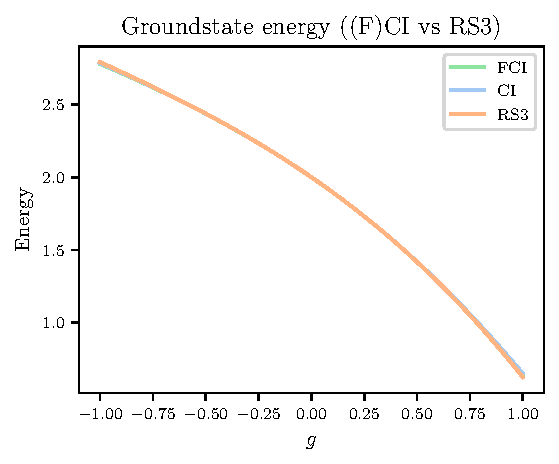
\includegraphics[width=\textwidth]{figures/e_groundstate_energy_RS.pdf}
        \caption{
            Groundstate energy from RSPT.\label{fig:rs_energy}
        }
    \end{subfigure}
    \hfill
    \begin{subfigure}[b]{0.5\textwidth}
        \centering
        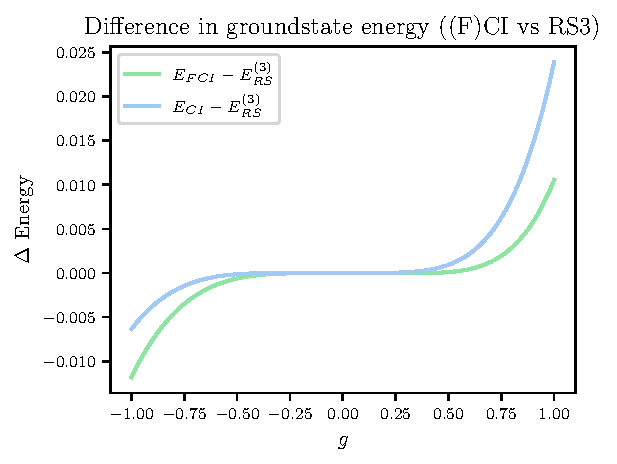
\includegraphics[width=\textwidth]{figures/e_groundstate_energy_diff_RS.pdf}
        \caption{
            Difference in energy from RSPT.\label{fig:rs_diff}
        }
    \end{subfigure}
    \caption{
        Groundstate energy from the Rayleigh-Schr\"odinger perturbation theory to third-order, compared with the FCI \& CI results, as a function of $g$.
    }
\end{figure}
